%%
%% This is file `sample-sigconf.tex',
%% generated with the docstrip utility.
%%
%% The original source files were:
%%
%% samples.dtx  (with options: `sigconf')
%% 
%% IMPORTANT NOTICE:
%% 
%% For the copyright see the source file.
%% 
%% Any modified versions of this file must be renamed
%% with new filenames distinct from sample-sigconf.tex.
%% 
%% For distribution of the original source see the terms
%% for copying and modification in the file samples.dtx.
%% 
%% This generated file may be distributed as long as the
%% original source files, as listed above, are part of the
%% same distribution. (The sources need not necessarily be
%% in the same archive or directory.)
%%
%% The first command in your LaTeX source must be the \documentclass command.
\documentclass[sigconf,a4paper]{acmart}

\usepackage{pgfplots}
\usepackage{tikz}
\usepackage{graphicx}
\usepgfplotslibrary{groupplots}
\pgfplotsset{compat=1.16}

%%
%% \BibTeX command to typeset BibTeX logo in the docs
\AtBeginDocument{%
  \providecommand\BibTeX{{%
    \normalfont B\kern-0.5em{\scshape i\kern-0.25em b}\kern-0.8em\TeX}}}

%% Rights management information.  This information is sent to you
%% when you complete the rights form.  These commands have SAMPLE
%% values in them; it is your responsibility as an author to replace
%% the commands and values with those provided to you when you
%% complete the rights form.
\setcopyright{acmcopyright}
\copyrightyear{2026}
\acmYear{2026}
\acmDOI{}

%% These commands are for a PROCEEDINGS abstract or paper.
\acmConference[DistAlg25/26]{The first project delivery of DistAlg25/26}{2026}{Faculdade de Ciências e Tecnologia, NOVA University of Lisbon, Portugal}
\acmBooktitle{The Projects of DistAlg - first project, 2026, Faculdade de Ciências e Tecnologia, NOVA University of Lisbon, Portugal}
\acmPrice{}
\acmISBN{}


%%
%% Submission ID.
%% Use this when submitting an article to a sponsored event. You'll
%% receive a unique submission ID from the organizers
%% of the event, and this ID should be used as the parameter to this command.
%%\acmSubmissionID{123-A56-BU3}

%%
%% The majority of ACM publications use numbered citations and
%% references.  The command \citestyle{authoryear} switches to the
%% "author year" style.
%%
%% If you are preparing content for an event
%% sponsored by ACM SIGGRAPH, you must use the "author year" style of
%% citations and references.
%% Uncommenting
%% the next command will enable that style.
%%\citestyle{acmauthoryear}

%%
%% end of the preamble, start of the body of the document source.
\begin{document}

%%
%% The "title" command has an optional parameter,
%% allowing the author to define a "short title" to be used in page headers.
% TODO
\title{Benchmarking Membership and Broadcast protocols in a distributed systems setting}

%%
%% The "author" command and its associated commands are used to define
%% the authors and their affiliations.
%% Of note is the shared affiliation of the first two authors, and the
%% "authornote" and "authornotemark" commands
%% used to denote shared contribution to the research.
\author{António Mendes}
\authornote{Student number 73530. Focus its work on implementing membership and broadcast protocols and cluster management for the evaluation criteria.}
\email{an.mendes@campus.fct.unl.pt}
\affiliation{%
  \institution{MEI, DI, FCT, UNL}
}

\author{Francisco Almeida}
\authornote{Student number 75116. Focus its work on developing our own gossip-based broadcast protocol.}
\email{fs.almeida@campus.fct.unl.pt}
\affiliation{%
  \institution{MEI, DI, FCT, UNL}
}

\author{Bernardo Gracioso}
\authornote{Student number 75486. Focus its work on implementing membership protocols and report writting.}
\email{b.gracioso@campus.fct.unl.pt}
\affiliation{%
  \institution{UCI, FCT, UNL}
}

%%
%% By default, the full list of authors will be used in the page
%% headers. Often, this list is too long, and will overlap
%% other information printed in the page headers. This command allows
%% the author to define a more concise list
%% of authors' names for this purpose.
\renewcommand{\shortauthors}{António, Francisco, and Bernardo.}

%%
%% The abstract is a short summary of the work to be presented in the
%% article.
\begin{abstract}
  This work evaluates the behavior of gossip-based broadcast protocols over different membership 
  overlays in a peer-to-peer distributed system, considering both fault-free execution and crash failures. 
  We compare three broadcast strategies - Flood, Eager Push, and Flare, a custom hybrid eager/lazy protocol 
  designed to reduce sender load by eagerly disseminating payloads to a subset of neighbors while allowing 
  remaining nodes to retrieve content via pull requests - evaluated over Full Membership, CYCLON, and HyParView 
  overlays in 100-node experiments with varying broadcast periods and payload sizes. Our results show that performance 
  depends strongly on the interaction between broadcast strategy and membership protocol: Flood achieves the highest 
  reliability but saturates the network under full membership, Eager Push delivers consistently low latency at the cost 
  of higher redundancy, and Flare successfully offloads the original sender while maintaining strong reliability even under 
  25\% node failures. However, Flare's load balancing depends heavily on the underlying overlay - CYCLON exposes pull-request 
  hotspots, while HyParView yields more stable distribution at the cost of higher membership overhead and tail latency. 
  Overall, no single combination dominates across all metrics, and the choice of protocol stack should be guided by the 
  application's priorities among reliability, latency, and communication overhead.
\end{abstract}


%%
%% This command processes the author and affiliation and title
%% information and builds the first part of the formatted document.
\maketitle

\section{Introduction}
Modern applications running on our mobile devices or even the emerging smart TVs rely 
heavily on distributed system architectures. If companies like Meta or Netflix ran their 
software on a single centralized server, they would fail to respond to thousands of client 
requests - the load is just too heavy for a single machine, leading to an increase in response 
times to their clients (or no response at all), and a higher probability of crashing.

This is why, in today's computing landscape, systems are divided into geographically dispersed 
nodes that communicate to achieve a common goal, following the architecture of distributed systems \cite{distributed_systems_principles_and_paradigms_2nd_edition}. 
This dispersal allows clients to be closer to the servers, resulting in lower response times, greater 
tolerance for machine failures (since data is replicated across several entities), and better load balancing.

Beyond traditional systems, some applications adopt a peer-to-peer (P2P) architecture. 
These systems must operate in a highly dynamic environment, where nodes frequently join 
and leave the network (high churn). A notable example is BitTorrent, a protocol that enables 
clients to download files faster through collaboration, where each node participates by uploading pieces 
of the file to other nodes while downloading it \cite{incentives-build-robustness-in-bittorrent}. Another example is crowdlending platforms, which allow 
individuals to lend money directly to others without relying on traditional financial institutions like banks, 
providing higher interest rates to investors \cite{P2P-lending-opportunities-and-risks}. This contrasts with applications, such as Netflix, which rely on 
centralized infrastructure and Content Delivery Networks (CDNs) to efficient distribution to their users, where 
servers are well-known and unlikely to change for a reasonable period of time \cite{measurement-study-of-netflix}.

For peer-to-peer systems to run correctly, nodes need to have a correct perception of 
the system's state, that is, the current active nodes, in order to propagate information 
across the network. Our project focuses on research into this topic, providing metrics 
on different implementations of protocols for materializing this concept and a discussion of the results obtained.


\section{Background}
A peer-to-peer system is a decentralized distributed system in which there is no central server, 
and all participating processes are equal, acting as both servers and clients simultaneously \cite{introduction-to-reliable-and-secure-distributed-programming}. 
The idea is that all participating peers share both the duties and the benefits of the system, 
collectively carrying out large-scale tasks that would require otherwise dedicated central servers, 
which would be more expensive. Peers jointly maintain an overlay network, a virtual network formed by 
processes (nodes) and the communication channels (links) between them, defined by logical relationships 
rather than physical presence or static connectivity, providing scalability to the system and the ability 
to handle high churn rates \cite{distributed_systems_principles_and_paradigms_2nd_edition,cyclon}.

Each node acts as both client and server \cite{distributed_systems_principles_and_paradigms_2nd_edition}, 
executing a common local algorithm \cite{introduction-to-reliable-and-secure-distributed-programming} 
(with its implementation shared across all peers in the network) to process and exchange information 
with others to achieve the common goal.

A node's behavior is often described as executing a protocol, which defines the format and legal 
sequences of messages exchanged with peers \cite{introduction-to-reliable-and-secure-distributed-programming}, portrayed 
as pseudo-code descriptions and specifications of the properties it wants to achieve. In many cases, a single process may execute a 
composition of multiple protocols \cite{babel_framework} that interact with their environment through an asynchronous 
event-based model \cite{distributed_systems_principles_and_paradigms_2nd_edition}. A protocol acts as an input consumer, processing various notifications and requests 
from local and remote sources, and as a producer of results from their internal computations and algorithmic 
logic, translated into messages received by other processes.

Based on how P2P systems manage their overlay network, they can be classified as: 
structured P2P systems, which use a deterministic procedure to organize nodes; 
or unstructured P2P systems, which rely on randomized algorithms to construct the overlay \cite{cyclon}. 
We focus on the latter category, since our work only examines the implementation of protocols for an 
unstructured overlay network.

Each node of an unstructured overlay maintains a list of neighbors, called their partial view, 
that is formed in a probabilistic way, such that it resembles a random graph, with low diameter 
(minimal distance between each pair of nodes, based on the short average distance), high resilience to 
failures and low clustering coefficient (that is, there are no observable self-contained groups of nodes). 
This collection represents a randomly chosen subset of nodes in the system, and ideally, choosing a node from 
it is equivalent to choosing one from the entire system, thereby imparting a uniform characteristic. \cite{distributed_systems_principles_and_paradigms_2nd_edition,cyclon}

For their functionality, P2P systems are built on two fundamental building blocks: 
membership management, in which nodes maintain a partial view of the system and keep it accurate by 
including only correct processes, thereby ensuring the overlay stays connected, providing a 
path between any two correct processes \cite{hyparview}. The second is broadcast or dissemination of information: 
when a node needs to inform all other nodes in the system, it starts by forwarding the message to a 
subset of its neighbors, following a gossip-based (epidemic) protocol \cite{distributed_systems_principles_and_paradigms_2nd_edition}.


\section{Implementation}

From a software engineering perspective, the protocols are implemented as software components or modules 
that are composed into software stacks. The interaction between protocols within a process is via message 
passing. Each layer produces and consumes several events: notifications/indications to the upper layers, 
indicating the delivery of information (for example, messages); and requests to other processes or layers 
to invoke a service at another component, which is generally related to a reply and is handled according 
to the logic. It also receives requests from the upper layers and can set up internal timers to execute 
periodic tasks. Each protocol has a state that is maintained through local variables, and because it is modeled 
as an event-driven state machine, the state only evolves through transitions triggered by the processing of events, 
managed by event handlers - code blocks responsible for executing the algorithm's logic \cite{introduction-to-reliable-and-secure-distributed-programming}.

We implement existing protocols using the Babel framework \cite{babel_framework}, optimized for quick prototyping and thus 
simplifying implementation without a significant performance impact. This Java framework follows an asynchronous, 
event-driven programming model and provides an API that serves as a natural bridge between the pseudo-code 
specifications and the code being written, while maintaining transparency by handling low-level operational 
complexities at the core.

This enables algorithmic specifications to be mapped almost line-for-line into Java implementations. 
At its core, Babel manages inter-protocol communication (both within the same process and across different processes). 
It handles event delivery to protocol event queues and abstracts the link between peers through a Channel class that, for example, 
supports TCP connection establishment, which was transversely used throughout the project.

\subsection{Project stack}

In our project, we consider an implementation stack that is described as follows from top to bottom: 
an application layer that makes requests to the underlying protocols, essentially for timing the dissemination 
of messages for collecting metrics of the overall performance and the overhead induced in the communication; 
the intermediary dissemination protocol, responsible for propagating those messages across the network; and 
finally the membership layer, for maintaining the awareness of the current peers participating in the network.

We started with the baseline code that the teacher João Leitão had provided to us, which already included 
implementations of the algorithms: BroadcastApp (application), FloodBroadcast (dissemination), and GossipBasedFullMembership 
(membership). This stack already provides the process with knowledge about the entire system, that is, all the nodes 
present in the overlay, and disseminates the requests to all known nodes.

\subsection{Membership protocols}

We followed by implementing CYCLON membership protocol (CyclonMembership) \cite{cyclon}, designed to build and maintain large-scale 
unstructured peer-to-peer overlays, where the partial view of a node has a fixed size and only contains a random 
sample of peers, that is maintained through affecting an age value to each entry on the view, and exchanging their 
partial views with other nodes by a shuffle request, also integrating the other node's own neighbors.

After that, we proceed to implement HyParView (HyParView\\Membership) \cite{hyparview}, a more complex membership protocol that uses two distinct 
partial views that are maintained by different strategies to ensure high reliability even during massive node failures.

\subsection{Broadcast protocols}

Above the membership layer, there is the dissemination or broadcast layer. In our project, we developed two more implementations: 
EagerPushGossipBroadcast and FlareBroadcast.

The dissemination strategy used in EagerPushGossipBroadcast is the same as in epidemic protocols \cite{epidemic-broadcast-trees}, where nodes immediately forward 
the full message payload to a random sample of peers they know from the membership (with a parameterized size, called fanout) upon receiving 
it for the first time.

\subsubsection{Self-Designed Gossip Broadcast}

Our Self-Designed Gossip Broadcast protocol is called Flare. Flare is a custom broadcast protocol designed to reduce the load placed on the original sender during message dissemination. Instead of eagerly sending the full payload to every known peer, Flare separates dissemination into two phases: an eager phase and a lazy pull-based phase.

When a node creates a broadcast message, it first selects a subset of its neighbors as the principal group. In our configuration, this corresponds to approximately 30% of the available neighbors. The sender transmits the full message payload only to this principal group. These nodes immediately deliver and store the payload, becoming additional owners of the message.

After receiving acknowledgments from the principal nodes, or after an acknowledgment timeout, the sender starts the lazy phase. In this phase, the sender contacts approximately 70% of the remaining neighbors with a lightweight metadata message. This lazy message does not contain the full payload. Instead, it contains the message identifier, the original sender, a TTL, and a list of nodes that are known to have the payload.

When a node receives a lazy message but does not yet have the payload, it chooses one of the advertised owners and sends a pull request. If the selected owner still has the payload stored, it replies with the full message. The requester then delivers the message locally and becomes a new owner. After receiving the payload, it can also forward lazy metadata to other neighbors, allowing the message to continue spreading without requiring the original sender to push the full payload to everyone.



\section{Evaluation}

To assess the effects of combining different layer implementations, we conducted experiments on the DI/NOVA LINCS Cluster. 
We created a virtual network of 100 nodes using oar-p2p, with Bonsai generating the 
corresponding network matrix for realistic latency. Experiments ran across charmander 1, 
charmander 2, and alakazam 8.

With the environment in place, we explored all possible combinations of membership and 
broadcast protocols. For each configuration, we varied the broadcast period (1000 ms and 3000 ms) 
and the payload size (20 bytes and 1000 bytes), leading to a total of 6 × 2 × 2 = 24 executions for 8 hours in total. 
Each run followed the same structure: an initial 45-second warm-up phase to stabilize the 
system, 120 seconds of active broadcasting, and 30 seconds to allow the network to drain 
any remaining messages. In addition, extra time was needed to deploy the nodes, terminate 
them, and gather the resulting logs.

During execution, each node recorded SEND and RECV events for each message ID. These logs 
served as the basis for our analysis.

To streamline the process, we used shell scripts to automate experiment execution and log 
collection across the cluster. The collected data was then processed in Python, generating 
CSV files containing the relevant metrics for further analysis.

The next subsections present our interpretation of the metrics, supported by a plot or table.

\subsection{Reliability}

When a process broadcasts a message, it aims to reach every peer in the overlay network. 
We can test whether this property is enforced by evaluating the ratio of the messages 
actually delivered to the expected number of deliveries, which equals the total messages 
sent. If the ratio is 1, the network can be considered reliable, meaning messages are never 
lost. But achieving perfection is only a theoretical concept, since practical protocols 
operate over fair-loss links \cite{introduction-to-reliable-and-secure-distributed-programming}; thus, no protocol stack reaches the 100\% barrier, as shown 
in the figure \ref{fig1}, even though it appears extremely close.

\begin{figure}[h]
  \centering
  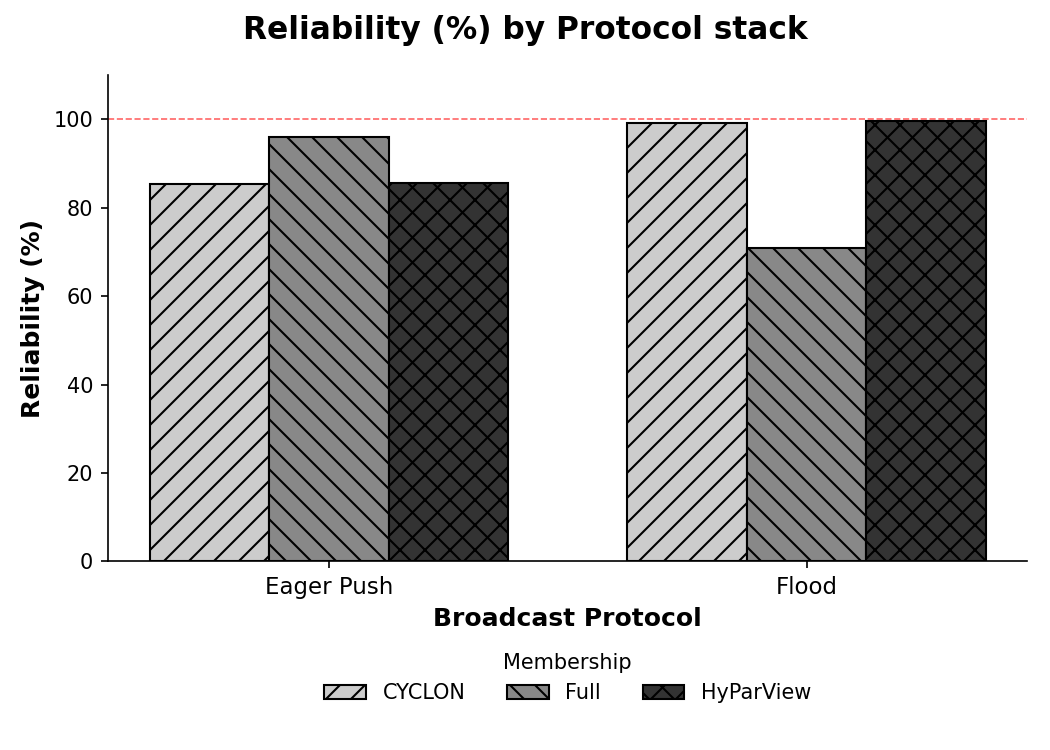
\includegraphics[width=\linewidth]{figures/reliability_bw.png}
  \caption{Reliability metric percentage evaluated on each protocol stack.}
  \Description{Reliability metric percentage evaluated on each protocol stack.}
  \label{fig1}
\end{figure}

One thing to consider is that the stacks built by the FloodBroadcast layer achieved better 
overall reliability than those built with EagerPushGossipBroadcast. The outcome is understandable 
because the specification of the eager push protocol explicitly states that the messages broadcast 
by correct processes are delivered by every correct process in the network with high probability if 
the parameterization is correct. Instead, the liveness property in the FloodBroadcast resembles the 
network flood, where the burden of reliability is entirely on the sender - if the sender is correct, 
the delivery to all other correct processes is guaranteed \cite{introduction-to-reliable-and-secure-distributed-programming}.

Another notable observation from the plot is that FloodBroadcast, when operating over the FullMembership layer, 
exhibits the lowest reliability. Although this may initially appear contradictory, it can be explained by considering 
the framework, where in this setup, Babel manages all communication between nodes using TCP channels. By maintaining a 
complete view of all nodes at the membership level and simultaneously employing a flooding strategy for message dissemination, 
the network becomes significantly overloaded. This excessive load causes TCP connection failures, leading to message loss and 
reduced delivery reliability. The composition is more effective when EagerPushGossipBroadcast operates on top of the 
FullMembership layer, because messages are disseminated to a small random subset of nodes from the entire network. 
In contrast, the other membership protocols maintain only a partial view of the network, limiting dissemination scope 
and reducing the probabilistic guarantees of message delivery.

\subsection{Latency}

The dissemination of messages is inherently constrained by latency arising from both physical 
and protocol-level factors. At the lowest layers of the network stack, data transmission occurs 
as signals, which require a non-negligible time to propagate across communication links.

We represented latency measurements using a boxplot \ref{fig2} to better visualize the 
data distribution. This representation is based on percentiles, statistical measures 
that indicate the value below which a given percentage of observations fall. The median 
(50th percentile) appears as the line inside the box, the first (Q1) and third (Q3) quartiles 
define the lower and upper bounds of the box, respectively, and additionally, the 95th and 99th 
percentiles, together with the minimum and maximum observed values, are included to capture the 
distribution's behavior.

\begin{figure}[h]
  \centering
  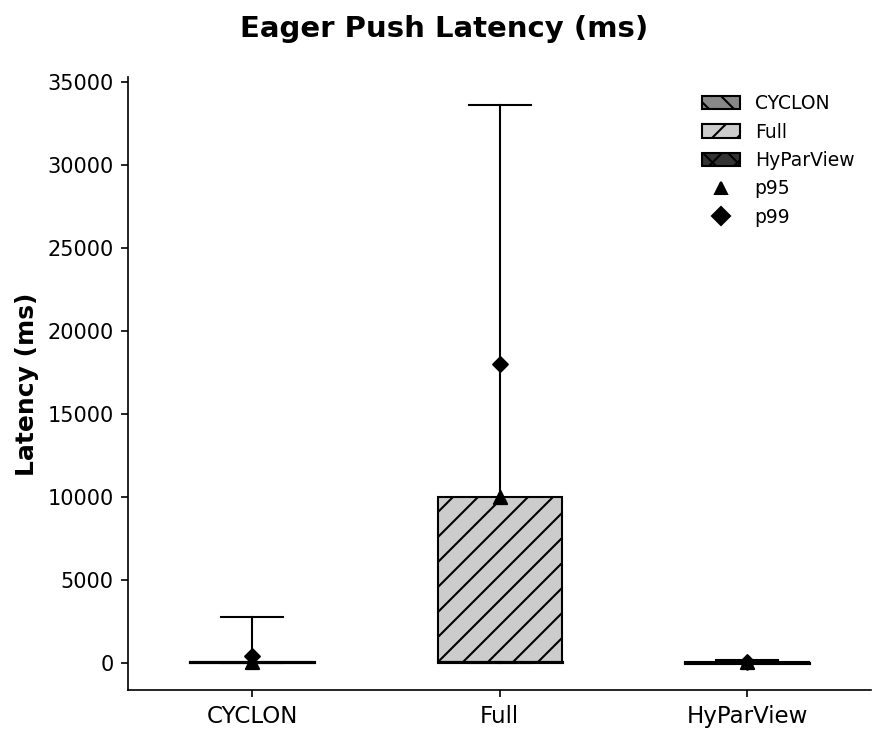
\includegraphics[width=0.7\linewidth]{figures/eagerpush_latency_boxplot_bw.png}
  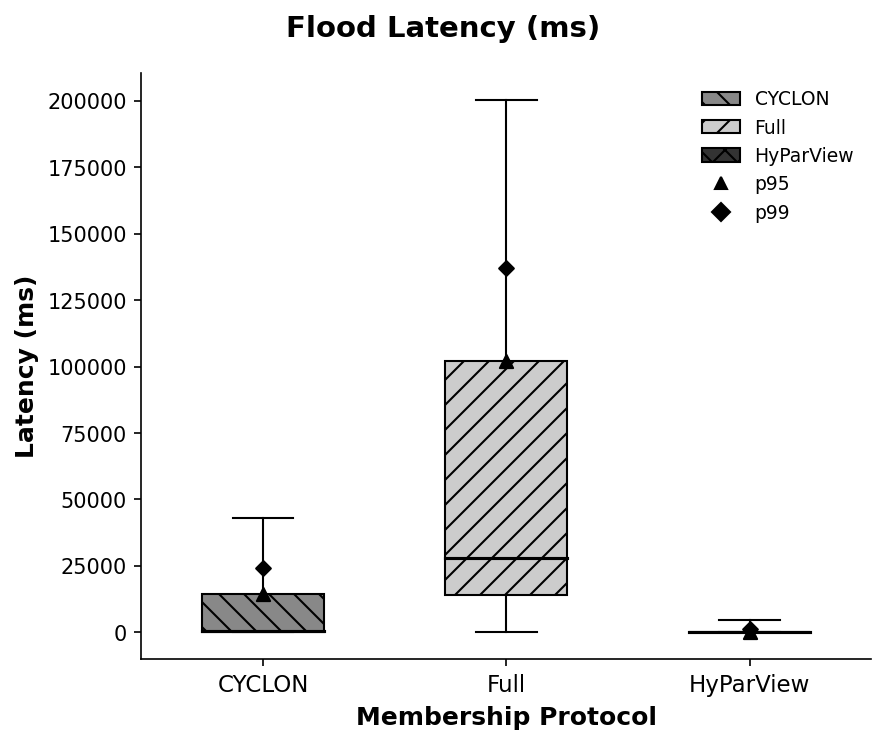
\includegraphics[width=0.7\linewidth]{figures/flood_latency_boxplot_bw.png}
  \caption{Latency in delivering broadcast messages on each protocol stack.}
  \Description{Latency in delivering broadcast messages on each protocol stack.}
  \label{fig2}
\end{figure}

Figure \ref{fig2} demonstrates that FullMembership exhibits the highest latency among the evaluated 
protocol stacks. The taller rectangle indicates greater dispersion of values, suggesting a much 
less consistent latency. This outcome is due to increased communication overhead: FullMembership 
requires more message exchanges, resulting in messages traversing more communication links. As 
each link introduces additional delay, and each link differs in the delay it injects, the 
cumulative effect produces both higher and more variable latencies.

In contrast, HyParView shows significantly lower latencies. This improvement is primarily due 
to the small and stable active view that it maintains, in which each node keeps an open TCP 
connection to every other node in its active view. Because this partial view is intentionally 
small, broadcast operations can be performed efficiently without overloading the network. 
This allows for a very fast failure detection: congested or unresponsive connections are 
quickly removed and replaced with peers from the passive view. As a result, the active 
view remains composed of relatively stable and well-performing links \cite{hyparview}.

When comparing broadcast strategies, eager push consistently achieves lower latency than 
flood broadcast. This difference is mainly explained by the number of messages propagated 
in each approach. Flood broadcast generates a significantly higher volume of messages, 
causing them to traverse a larger number of network links. Because each link introduces 
its own transmission delay, this results not only in higher overall latency but also in 
greater variability in delivery times. On the other hand, eager push reduces the number 
of transmissions to a smaller set of peers, limiting the number of links involved in message 
dissemination, leading to more consistent and overall lower latency.

\subsection{Redundancy}

In a Flood-based dissemination strategy, every node transmits messages to all other nodes. 
This results in high redundancy, as we can see in table \ref{tab:broadcast_membership} since multiple copies of the same message traverse the network 
through different paths. While this increases reliability in theory, it can also introduce 
significant communication overhead.

When FloodBroadcast is combined with a FullMembership layer, in which every node maintains 
connections to all other nodes, the network becomes highly susceptible to overload. Because 
all nodes attempt to communicate with all others simultaneously, this leads to congestion, 
connection failures, and ultimately message loss. Despite its high redundancy, this 
configuration can exhibit low reliability in practice. On the other hand, gossip-based 
approaches such as EagerPushGossipBroadcast reduce redundancy by disseminating messages 
to only a subset of peers.

Membership protocols also play a key role. CYCLON constructs a random and connected overlay, 
ensuring that nodes maintain a partial and randomized view of the network. This promotes 
robustness and randomness in message dissemination. In contrast, HyParView uses a more robust 
overlay, maintaining active and passive views to ensure connectivity while minimizing overhead. 
This design results in lower redundancy and more efficient communication than fully connected 
approaches.

Finally, combining Eager Push gossip with membership overlays (such as CYCLON or HyParView) 
typically results in a better trade-off between reliability and scalability. These approaches 
avoid the excessive redundancy of flooding while still achieving a high probability of message 
delivery, especially in large-scale distributed systems.

\begin{table}[h]
\centering
\begin{tabular}{lll}
\hline
\textbf{Broadcast} & \textbf{Membership} & \textbf{Redundancy (\%)} \\
\hline
Eager Push & CYCLON & 85.57 \\ Eager Push & Full & 96.31 \\ Eager Push & HyParView & 12.45 \\ Flood & CYCLON & 98.91 \\ Flood & Full & 65.06 \\ Flood & HyParView & 49.51 \\
\hline
\end{tabular}
\caption{Broadcast vs Membership Redundancy}
\label{tab:broadcast_membership}
\end{table}

\subsection{Membership overhead}

The results in Table \ref{tab:membership-overhead} highlight a clear trade-off between 
control-plane overhead and overlay robustness across the evaluated membership protocols.

The Full membership protocol exhibits the lowest overhead in both messages per second and bytes 
per second. This is expected, as each node maintains a complete view of the network with minimal 
active maintenance. However, this design does not scale well in dynamic or failure-prone 
environments, since maintaining global consistency becomes increasingly expensive and fragile 
as churn increases.

CYCLON introduces a moderate increase in overhead compared to Full membership. This aligns 
with its gossip-based design, where nodes periodically perform shuffle exchanges to maintain 
a randomized partial view of the network. These periodic exchanges generate additional control 
messages, but they avoid the global synchronization cost of Full membership. As a result, 
CYCLON represents a balanced approach, trading a modest increase in maintenance cost for 
improved adaptability and scalability in large-scale unstructured overlays.

In contrast, HyParView generates significantly higher overhead by orders of magnitude in 
both messages and bytes per second. This is due to its dual active/passive view structure 
and continuous view maintenance mechanisms, including frequent updates and failure detection 
operations. Although this introduces substantial bandwidth and processing costs, it is a 
deliberate design choice. In gossip-based peer-to-peer systems, this additional control 
traffic supports rapid recovery from failures and strong resilience under high churn, which 
is often critical in unreliable distributed environments.

\begin{table}[h]
\centering
\begin{tabular}{lrr}
\toprule
\textbf{Protocol} & \textbf{Messages/s} & \textbf{Bytes/s} \\
\midrule
CYCLON     &    88.825 &   4{,}380.125 \\
Full       &    52.850 &   2{,}094.450 \\
HyParView  & 4{,}166.050 & 191{,}480.175 \\
\bottomrule
\end{tabular}
\caption{Membership Overhead per Second by Protocol}
\label{tab:membership-overhead}
\end{table}



\subsection{Flare}

Flare maintains its main design goal even under crash conditions: most payload bytes are delivered via pull replies rather 
than eager push. As a result, it effectively offloads traffic from the original sender and 
the principal dissemination group.

In terms of reliability, Flare remains viable under failure scenarios. Even with up to 25\% 
node crashes \ref{fig3}, it achieves strong delivery consistency. Its reliability is slightly below 
Flooding but clearly better than Eager Push in most crash configurations. This confirms 
that Flare's hybrid push-pull design is robust under churn and failures.

However, load-balancing results are more nuanced and depend heavily on the underlying 
membership layer. We used a Gini \ref{tab:combined-performance} coefficient as a way to measure load balancing
across the system. With HyParView and Full Membership, Flare achieves acceptable—but not 
exceptional—load distribution. The busiest node still handles roughly 4x-5x the average payload 
load, indicating some residual skew in request ownership and pull coordination.

The situation changes significantly when using CYCLON. While Flare combined with CYCLON maintains 
a high fraction of pull-based payload delivery, it introduces a pronounced load imbalance: the 
most heavily loaded node can send approximately 33.71x the average payload traffic. This 
confirms a previously observed issue under fault-free conditions: although CYCLON provides 
good reachability and uniform randomness at the membership level, Flare's current owner-selection 
and pull coordination logic can concentrate requests on a small subset of nodes, creating hotspots.

Overall, this highlights a key trade-off in Flare's design. CYCLON improves randomness and 
reachability in the membership layer but exposes weaknesses in the broadcast/pull ownership 
mapping. In contrast, HyParView produces significantly better load distribution when paired 
with Flare, resulting in the most balanced configuration among the evaluated setups.

Flare's most consistent strength across all configurations is its ability to shift traffic away 
from eager dissemination. The pull-based design ensures that the original sender does not need 
to transmit full payloads to all nodes; instead, it seeds the message to a smaller principal 
group. The remaining nodes then retrieve the payload through pull requests, distributing 
transmission responsibility across the system.

The main cost of this design is latency. Flare can achieve relatively fast dissemination under 
CYCLON due to its aggressive randomness, but with HyParView and Full Membership, tail latency 
increases. This is largely due to the additional indirection introduced by the pull phase: 
nodes first receive metadata, then issue pull requests, and finally wait for responses. 
Under high load or failure conditions, this multi-step process can amplify delays.

In summary, Flare clearly succeeds as a sender-offloading gossip protocol, but its performance 
depends heavily on the composition of underlying layers. It reduces eager push overhead and 
remains reliable under crashes, yet it does not inherently guarantee balanced load distribution. 
Instead, its efficiency and scalability are strongly shaped by how well the membership layer 
aligns with its pull-based ownership strategy.

\begin{figure}[h]
  \centering
  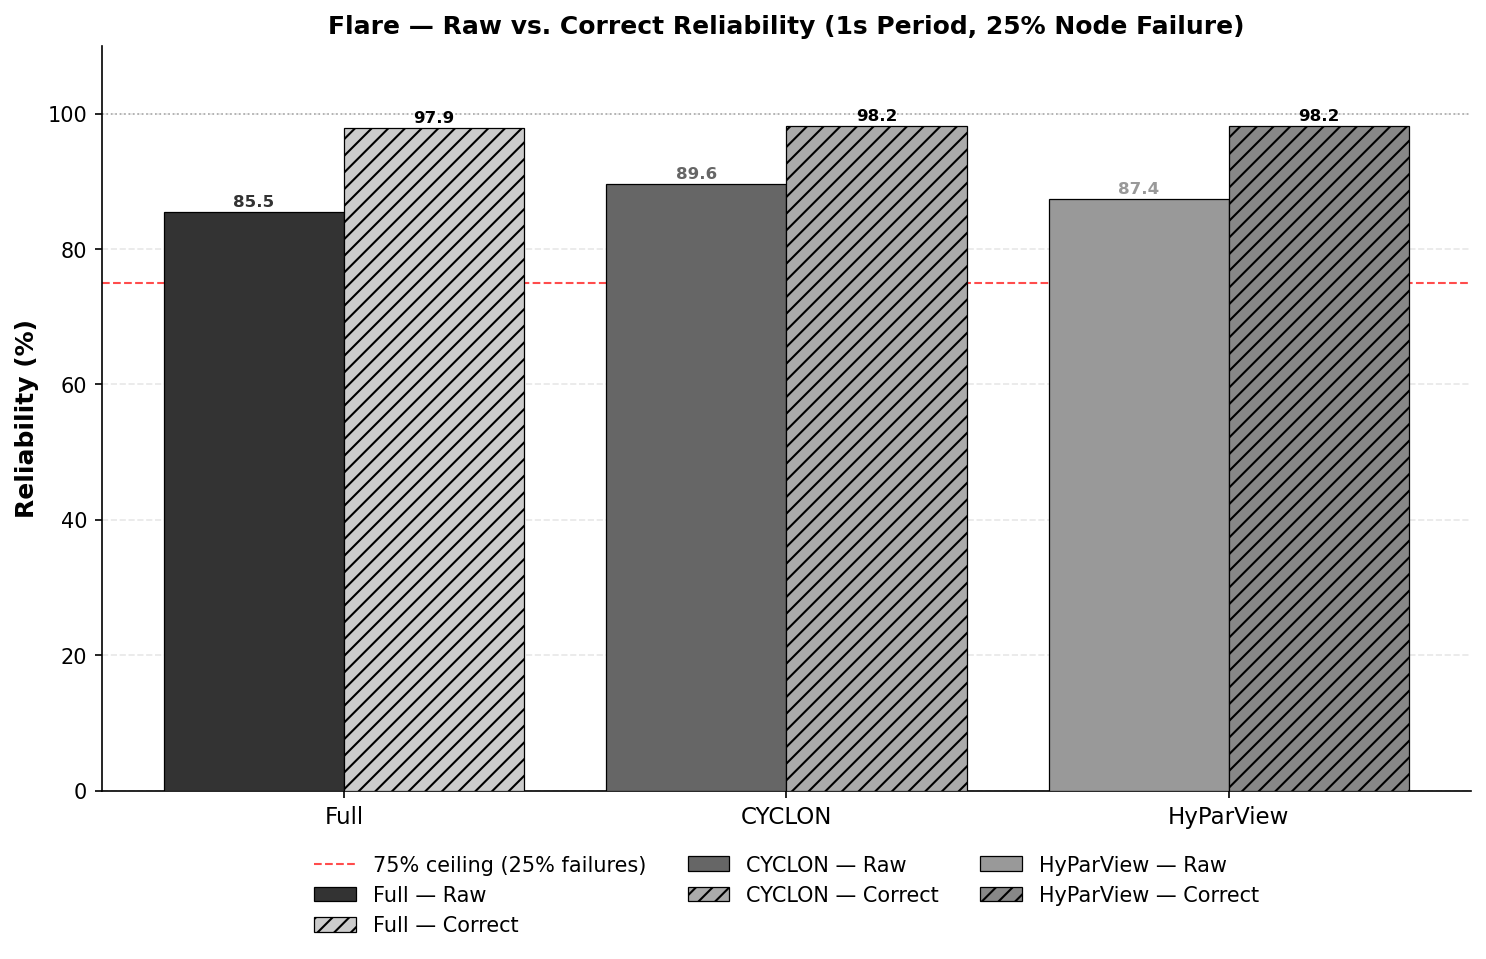
\includegraphics[width=\linewidth]{figures/flare_raw_vs_correct_reliability_1s_bw.png}
  \caption{Flare reliability under 25\% node failure (1s broadcast period).}
  \Description{Flare reliability under 25\% node failure (1s broadcast period).}
  \label{fig3}
\end{figure}

\begin{table}[h]
\centering
\resizebox{\columnwidth}{!}{%
\begin{tabular}{lrrrr}
\toprule
\textbf{Protocol} & \textbf{p95 Latency (ms)} & \textbf{Max/Avg Load (Gini)} & \textbf{Reliability (\%)} & \textbf{Pull Payload (\%)} \\
\midrule
CYCLON     &    20.5 & 33.71x\ \ (0.600) & 98.161 & 95.68 \\
HyParView  & 17{,}033.8 &  4.33x\ \ (0.530) & 98.828 & 87.53 \\
Full       & 32{,}309.2 &  5.33x\ \ (0.503) & 98.005 & 82.92 \\
\bottomrule
\end{tabular}%
}
\caption{Performance comparison across latency, load balancing, reliability, and crash resilience}
\label{tab:combined-performance}
\end{table}

\section{Conclusion}

The evaluation of Flooding and EagerPush broadcast protocols reveals clear trade-offs between 
reliability, latency, and failure recovery, which are directly linked to the underlying 
membership protocol.

Building on this, Flooding achieves very high reliability, around 99\%, when used with 
protocols such as CYCLON and HyParView. However, it performs poorly under full membership, 
especially at higher broadcast rates. In these cases, excessive message redundancy leads to 
network congestion and significant reliability degradation. Despite this limitation, Flooding 
remains robust under failures and maintains high delivery rates among correct nodes.

EagerPush, on the other hand, provides consistently low latency across all configurations, 
making it the fastest protocol evaluated. However, its reliability is significantly lower 
than Flooding, particularly under failures, where it suffers substantial degradation due to 
the absence of any recovery mechanism for lost messages.

The choice of membership protocol is critical. Full membership further exacerbates scalability 
issues in Flooding, but benefits EagerPush by improving connectivity. CYCLON performs well in 
Flooding but shows weaker reliability under failures in EagerPush. HyParView provides the best 
overall balance, combining high reliability and low latency, particularly for Flooding.

The evaluation of the Flare broadcast protocol with different membership algorithms further 
reinforces that the membership structure is key to the efficiency and overall operation of 
the system, especially under heavy loads and failure conditions. In the failure-free case, 
both CYCLON and HyParView maintain consistently high reliability rates, around 99\%, while 
full membership performs significantly worse at higher broadcast rates due to network congestion. However, increasing the broadcast period helps mitigate this effect, with full membership stabilizing at reliability levels closer to the other configurations.

Under node failures, all configurations maintain high reliability among correct nodes, demonstrating
 Flare's robustness and the benefits inherited from the underlying membership protocols. 
 In terms of latency, CYCLON performs best compared to HyParView and full membership, as 
 its random gossip-based structure enables faster dissemination. In contrast, HyParView and 
 full membership experience higher delays due to more structured communication patterns and 
 increased overhead.

As expected, network cost analysis shows that Flare relies heavily on pull-based recovery, 
with the majority of requests originating from pull replies. CYCLON exhibits poorer load 
balancing compared to HyParView and full membership, which distribute communication 
load more evenly across nodes. Overall, HyParView offers the best trade-off between reliability, 
load balancing, and robustness, while CYCLON achieves the lowest latency at the cost of fairness. 
Full membership is only competitive under low broadcast rates due to its scalability limitations.

Additionally, increasing the period consistently reduces the broadcast rate, thereby improving 
reliability and stability across both protocols. This highlights the impact of network congestion 
on performance.

In summary, Flooding is preferable when reliability is the primary concern and partial 
membership is used, while EagerPush is better suited for latency-sensitive scenarios where 
occasional message loss is acceptable. Across both protocols, HyParView consistently emerges 
as the most balanced membership solution, particularly under failure conditions and varying load.

%%
%% The next two lines define the bibliography style to be used, and
%% the bibliography file.
\bibliographystyle{ACM-Reference-Format}
\bibliography{sample-base}

\end{document}
\endinput
%%
%% End of file `sample-sigconf.tex'.
